\documentclass[11pt, onecolumn]{article}
\usepackage{hyperref}
\usepackage{url}
%\usepackage{mathpazo,mathrsfs}
%\usepackage[T1]{fontenc}

%\usepackage[usenames,dvipsnames]{color}
\usepackage{stmaryrd} \usepackage{url} \usepackage[latin1]{inputenc}
\usepackage{graphicx}% Include figure files
\usepackage{amssymb} \usepackage{subfigure} \usepackage{amsmath}
\usepackage{amsthm}
\usepackage{dcolumn}% Align table columns on decimal point
\usepackage{bm}% bold math
\usepackage{color}
\usepackage{mathtools}


%\usepackage{algorithm} \usepackage{algorithmic}
\usepackage[noline,boxed]{algorithm2e}

\newcommand{\alert}[1]{\textcolor{red}{#1}} \newcommand{\vect}[1]{\boldsymbol{#1}}
\newcommand{\todo}[1]{\vspace{5 mm}\par \noindent \framebox{\begin{minipage}[c]{8cm} \tt
      #1
    \end{minipage}}\vspace{5 mm}\par}

\newcommand{\STATE}{\quad}
\newcommand{\COMMENT}[1]{{\sl (#1)}}
\newcommand{\RETURN}{\tb{Return }}

\newtheorem{theorem}{Theorem}[section]
\newtheorem{statement}[theorem]{Statement}
\newtheorem{proposition}[theorem]{Proposition}
\newtheorem{lemma}[theorem]{Lemma}
\newtheorem{corollary}[theorem]{Corollary}
\newtheorem{question}[theorem]{Question}
\newtheorem{remark}[theorem]{Remark}
\newtheorem{conjecture}{Conjecture}
\newtheorem{claim}[theorem]{Claim}
\newtheorem{condition}[theorem]{Condition}
\newtheorem*{subproblem*}{Subproblem}
\newtheorem{definition}[theorem]{Definition} \newtheorem{example}{Example}
\newtheorem{assumption}{Assumption} \newtheorem{scenario}{Scenario}
\newtheorem{step}{Step} \newtheorem{steps}{Step} \newtheorem{stp}{Step}
\newtheorem{stps}{Step} \newtheorem{problem}{Problem}

%\newenvironment{proof}[1][Proof]{\begin{trivlist}
%\item[\hskip \labelsep {\bfseries #1}]}{\end{trivlist}}


\usepackage{hyperref}

%\renewcommand{\algorithmicrequire}{\textbf{Input:}}
%\renewcommand{\algorithmicensure}{\textbf{Output:}}
%\renewcommand{\algorithmireturn}{\textbf{Return:}}



%\usepackage[dvips]{graphicx}
% \usepackage{amsfonts,mathrsfs,amsfonts, array, geometry}
% \usepackage{graphicx,amsmath,amssymb,multirow} \setcounter{MaxMatrixCols}{30}%
% \usepackage[usenames]{color} \usepackage[usenames, dvipsnames]{xcolor}
% \usepackage{epstopdf}\usepackage{framed}
% \usepackage{algpseudocode}
% \usepackage{ulem}

% \newtheorem{Thm}{Theorem} \newtheorem{Lem}{Lemma} \newtheorem{Cor}{Corollary}
% \newtheorem{Def}{Definition} \newtheorem{Exam}{Example} \newtheorem{Alg}{Algorithm}
% \newtheorem{Prob}{Problem} \newtheorem{Rem}{Remark} \newtheorem{Proof}{Proof}
% \newtheorem{Prop}{Proposition} \newtheorem{Assump}{Assumption}

\newcommand{\mc}{\mathcal}
\newcommand{\mb}{\mathbf} \newcommand{\mbb}{\mathbb} \newcommand{\wt}{\widetilde}
\newcommand{\fa}{\forall} \newcommand{\tc}{\textcolor} \newcommand{\tb}{\textbf}
\newcommand{\tx}{\text} \newcommand{\tcws}{\textcolor{WildStrawberry}}
\newcommand{\tcbl}{\textclor{blue}}
\newcommand{\p}{\partial}
\newcommand{\dr}{\text{d}}
\newcommand{\bs}{\boldsymbol}
\newcommand{\ot}{\otimes}

\newcommand{\ta}{\theta}
\newcommand{\Ta}{\Theta}

\newcommand{\Proj}{\mbox{Proj}}
\newcommand{\R}{\mbb R}
\newcommand{\C}{\mbb C}
\newcommand{\Z}{\mbb Z}
\newcommand{\E}{\mbb E}

\newcommand{\ul}{\underline}
\newcommand{\ol}{\overline}
\newcommand{\wh}{\widehat}
\newcommand{\prj}{\tx{Proj}}
% \newcommand{\mog}{Gaussian mixture model}
\newcommand{\mog}{mixture of Gaussians }
% \newcommand{\mog}{MoG}
\newcommand{\vc}{\tx{vec}}
\newcommand{\mt}{\tx{mat}}
\newcommand{\diag}{\tx{diag}}
\newcommand{\poly}{\tx{poly}}
\newcommand{\cond}{\tx{cond}}
\newcommand{\ep}{\tx{exp}}
\newcommand{\lt}{\left}
\newcommand{\rt}{\right}

\newcommand{\defeq}{\vcentcolon=}
\newcommand{\eqdef}{=\vcentcolon}
\newcommand{\od}{\odot}

%\linespread{1}
%\let\labelindent\relax
\usepackage{enumitem}
\usepackage[margin=1in]{geometry}

\newcommand{\qq}[1]{{\color{magenta}{(#1)}}}
\newcommand{\rd}[1]{{\color{red}{ #1}}}
\newcommand{\bl}[1]{{\color{blue}{ #1}}}
\iffalse
\fi

\begin{document}
\title{controller validation for uncertain systems}
\date{\today}

%\maketitle
%\thispagestyle{empty}
%\pagestyle{empty}

% \begin{abstract}
% \end{abstract}
% \begin{keywords}
% \end{keywords}

\setcounter{page}{1}


\section{ID-Control Problem}
The goal is to use IQC constraints to replace the clear-cut between sys id and robust controller
synthesis.


\paragraph{To do list }
\begin{enumerate}
\item
  simulation of the simple setting to see how it works (with IQC synthesis)
\item
  sample complexity of controller invalidation
\item
  sample complexity of robust controller synthesis
\end{enumerate}



\paragraph{Step 1, sys id}
Open loop id for unknown plant $P$. Run experiment to obtain (input, output) sequence
$(s,v)$.
\begin{figure}[!ht]
  \centering
  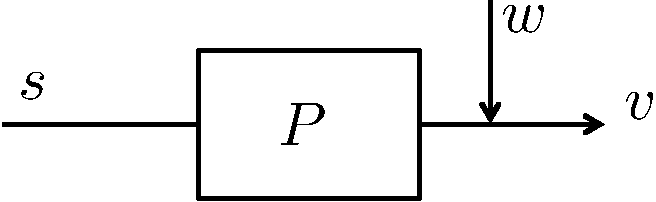
\includegraphics[width=.3\linewidth]{sys3.pdf}
\end{figure}

Assume the measurement noise $w$ in a bounded set with IQC description $\mc Q_w$. Convert the
observation $(s,v)$ to IQCs about the plant.

For example, assume that $P$ is FIR and the length of the observation is larger, and assume that $w$
lies in bounded $\ell_2$ ball. We parameterize the plant by its impulse response $p$.  The observation
$(s,v)$ gives the following constraint on $p$:
\begin{align*}
  \| v - p*s\|_2\le \gamma_w.
\end{align*}

\paragraph{Step 2, controller invalidation}

Place the candidate controller $K$ in the closed loop. Run experiment to obtain (reference, output)
sequence $(r, y)$.
\begin{figure}[!ht]
  \centering
  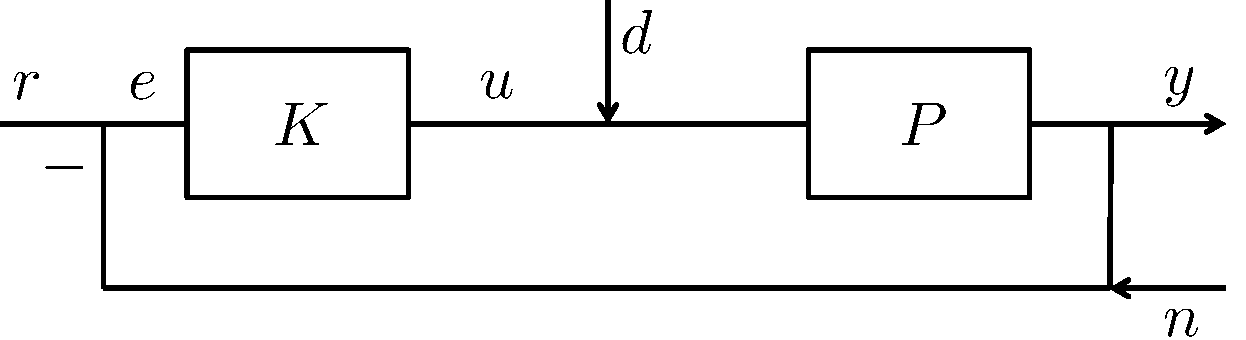
\includegraphics[width=.5\linewidth]{sys2.pdf}
\end{figure}

Given the constraints for the uncertain plant from Step 1, the disturbance $d$ and the measurement
noise $n$ as $\mc Q_d$, $\mc Q_n$. Let $\mc Q_{T,\gamma}$ denote the achieved quadratic performance
of the closed loop channel $r\to y$ with parameter $\gamma$.

The invalidation of controller $K$ is to certify that there does not exist noise signal $(d, n)$ and
impulse response of the plant $p$ such that:
\begin{align*}
  & (r,y)\in\mc Q_{T,\gamma}, \quad\tx{(tracking performance achieved)}
  \\
  & e = r-(y+n), \quad u = K e, \quad y = p * (u+d),  \quad\tx{(signals)}
  \\
  & d\in\mc Q_d, \quad n\in\mc Q_n,  \quad (v-p*s )\in\mc Q_w. \quad\tx{(constraints satisfied)}
\end{align*}

Set $\mc Q_d$ and $\mc Q_n$ to be $\ell_2$ ball, and parameterize $K$ by a FIR $k$.  We invalidate $K$
if there does not exist signal $(d, n, p )$ such that
\begin{align*}
  & e = r-(y+n), \quad u = k * e, \quad y = p * (u+d), \quad\tx{(signals)}
  \\
  & \|y - r\|_2 \le \gamma, \quad \|d\|_2\le \gamma_d, \quad  \|n\|_2\le \gamma_n, \quad
  \|v-p*s\|_2\le \gamma_w.
\end{align*}
\qq{convex?}

In the parlance of Smith and Dullerud, we have
\begin{align*}
P \triangleq &\; \bmat{-I & I & -I & K\\I & 0 & 0 & 0}\\
\Delta \triangleq &\; p \\
u \triangleq &\; r \\
w \triangleq &\; \bmat{d\\n}\\
W_0(w) = &\; \gamma_d^2 - ||d||_2^2\\
W_1(w) = &\; \gamma_n^2 - ||n||_2^2\\
Q_1(z,v) = &\; \text{ some constraint on $p$?}
\end{align*}


\tb{ Sample complexity question.}
Suppose $K$ can be invalidated. Assume that $w$, $d$, $n$ are Gaussian white noise. How many
roll-outs in Step 1 do we need in order to invalidate $K$ with high probability.


\paragraph{Step 3, robust controller synthesis}
The synthesis problem of $K$ is as follows:
\begin{align*}
  &\min_{K\in\mc K} \gamma,\quad s.t. \tx{ the above inequalities hold}.
\end{align*}
Note that this is  nonconvex.

\tb{ Sample complexity question.}
Assume that $w$, $d$, $n$ are Gaussian white noise. How many roll-outs in Step 1 do we need in order
to find $K$ sufficiently close to the optimal controller with respect to the underlying true plant.



% Given $M$ observed roll-outs for step 1, we can obtain tighter constraints of $P$, which converges
% to the underlying truth, and the optimal solution in the second step also converges to the optimal
% controller with respect to the true plant $P$. Establish the asymptotic convergence, and then finite
% sample rate.

% \paragraph{Naive questions}
% Why not replace Step 2 with IQC synthesis? why not replace Step 1 with point estimator plus
% uncertainty set? Advantage compared to existing 2-step ID and robust control?


\newpage



\section{Controller invalidation for synthesis}
Robust synthesis is non-convex.  If we can do experiments to test different controllers, can we
``solve'' the synthesis problem by ruling out controllers which do not achieve the robust
performance? How to design the experiments to ``solve'' the synthesis problem in a more efficient
way?

%Decreases complexity by introducing uncertainty to the system and be more conservative.

\paragraph{To do list }
\begin{enumerate}
\item Find a simple parameterization of controller such that it works.
\item Sample complexity of invalidation?
\item Iterative id and invalidation?
\end{enumerate}



\paragraph{Setting}
Given:
\begin{itemize}
\item The part of plant that is known a priori, denoted by $P$.
\item Support of the of the unknown part of the plant $\Delta$: an {\em initial} description in the
  form of integral quadratic constraints on its input-output pair $(v,s)\in \mc Q_\Delta =
  \{Q_1,\dots, Q_L\}$.
  % (why not ssv or coprime factor)
\item Support of the controller $K$: a (discrete) set of candidate controllers $K \in \mc K =
  \{K_1,\dots, K_M\}$.
\item Support of the unobserved exogenous noise $w$: a bounded set in the form of IQCs $w\in \mc
  Q_{w}$.
\end{itemize}
Goal: find a controller $K\in\mc K$ that achieves robust stability and performance.

\paragraph{Basic idea}
The basic idea of ``controller invalidation experiments for synthesis'' is as follows.

Consider closed-loop system with a candidate controller $K\in\mc K$ in place.  Generate length $T$
observation $(u_t, y_t, z_t)_{t=1}^{T}$ generated by the closed loop system.

  Given $P, \mc Q_{\Delta}, \mc Q_{W}$, invalidate $K$ if there does not exist signal $(w_t, v_t,
  s_t)_{t=1}^{T}$ such that the following holds:
\begin{enumerate}
\item
  \begin{align*} (z,y,v) = P (u,w,s), \quad u = K z.
  \end{align*}
  Let $F_u(P,K)$ denote the linear fractional transformation, the two time domain equalities are
  equivalent to
  \begin{align*} (y,v) = F_u(P,K) (w,s).
  \end{align*}

\item IQCs for system  uncertainties are satisfied:
  \begin{align*} & w\in\mc Q_w, \quad (v,s) \in \mc Q_{\Delta}
  \end{align*}

\item Performance achieved.
  \begin{align*}
    (w,y) \in \mc Q_{T, \gamma}.
  \end{align*}
\end{enumerate}
\qq{convex?}

We need to do this test for every $K$ in the discrete set $\mc K$ to determine whether to keep it or
throw it out. If more than one $K$ is left, try:
\begin{itemize}
\item Get new observations for each $K$ with the same setup. Run the same invalidation procedure.
\item With the same observation, search for better performance so that sub-optimal controllers would
  be ruled out.
\end{itemize}



\begin{figure}[!ht]
  \centering
  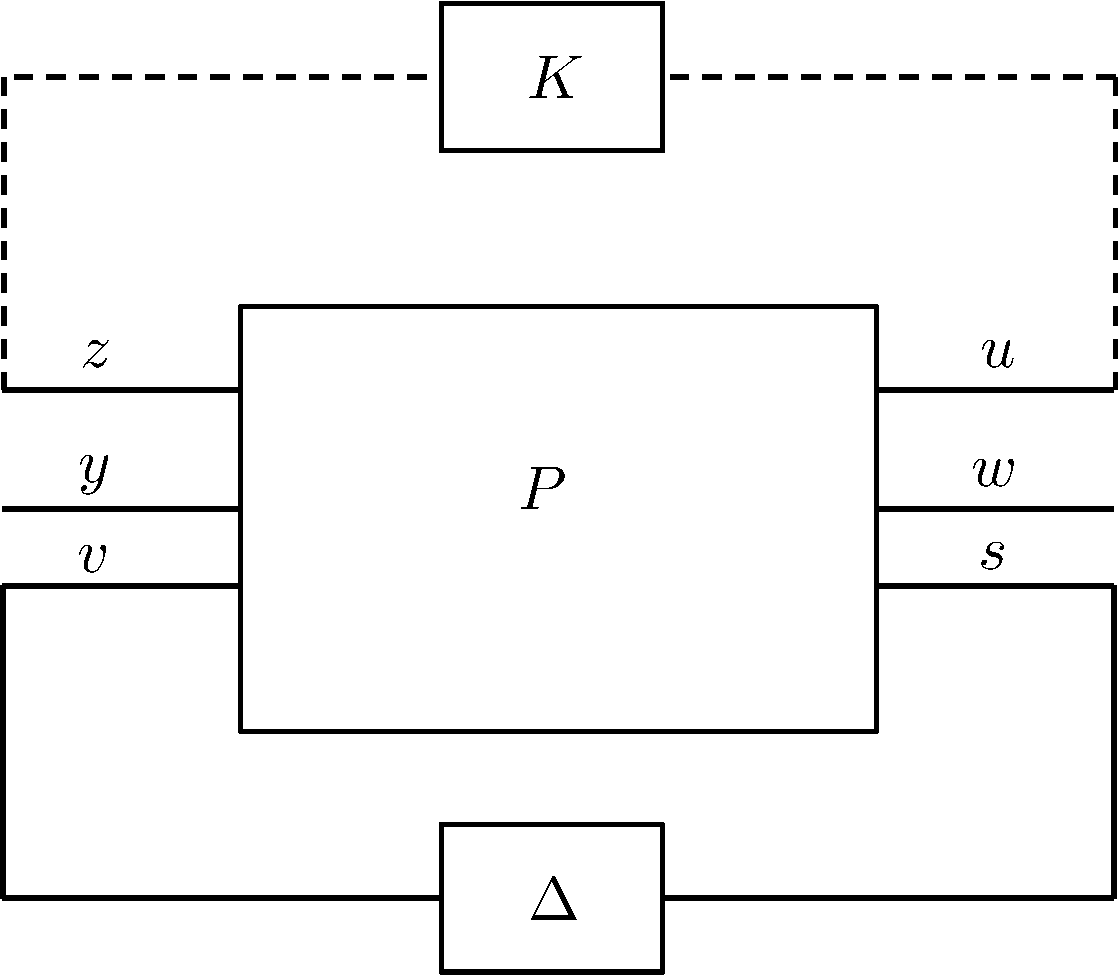
\includegraphics[width=.4\linewidth]{sys1.pdf}
\end{figure}




\paragraph{Discussions}
\begin{enumerate}
\item Start with a compact set for $\mc K$, we want to test one instance of $K$ and be able to rule
  out a measurable subset of $\mc K$.

  Experiment design. Note that in the closed loop id, choosing a particular controller $K$
  determines the $u$ input sequence. We want to select a controller $K\in \mc K$ so that we can
  shave of a large portion of $\mc K$ with the invalidation procedure.

\item Incorporate the information in the observed sequences to get a finer description of the
  uncertainty set $\Delta$, which would give us more invalidation power.

 For each $K_i\in\mc K$, we can potentially identify a set of $\Delta$ that are consistent with
  the observation for some $w\in\mc Q_{w}$. Denote it by $\Delta_{K_i}$.
  \\
  Find the tightest IQC description for the set $\cap_i \Delta_{K_i}$ and denote it by $\mc
  Q_{\Delta}'$.  Can we confidently rule out the subset of $\Delta$ in $\mc Q_{\Delta} \backslash
  \mc Q_{\Delta}'$?  No system in this subset can generate the observed sequences.


\end{enumerate}






\bibliographystyle{plain}
\bibliography{invalid}

\end{document}
